\documentclass[10pt,letterpaper]{article}
\usepackage[margin=1in]{geometry}
\usepackage{amsmath,amssymb}
\usepackage{booktabs}
\usepackage{graphicx}
\usepackage{hyperref}
\usepackage{xcolor}
\usepackage{enumitem}
\usepackage{multirow}
\usepackage{algorithm}
\usepackage{algpseudocode}
\usepackage{listings}
\usepackage{caption}
\usepackage{subcaption}

% paper/macros.tex
% LaTeX macros for numbers used across the paper and CHECKLIST.md.
% Shared so the paper and checklist cannot drift (#65 acceptance criterion).

% --- Pinned stack (#57) ---
\newcommand{\vllmVersion}{0.25.1}
\newcommand{\torchVersion}{2.11.0+cu130}
\newcommand{\gpuModel}{NVIDIA A100 80GB PCIe}

% --- Quality (#43 rescore, 9-field) ---
\newcommand{\arThreeBFnine}{0.8516}   % AR-3B at L=256, 9-field F1
\newcommand{\dgNineF}{0.8518}         % DG at L=256, 9-field F1
\newcommand{\arThreeBFtwelve}{0.8263}  % AR-3B at L=256, 12-field F1
\newcommand{\dgTwelveF}{0.7858}        % DG at L=256, 12-field F1

% --- Cost laws (Campaign B, pending re-measurement on pinned stack) ---
\newcommand{\arBase}{7.27}       % AR-3B fitted intercept (ms)
\newcommand{\arSlope}{6.29}      % AR-3B ms per output token
\newcommand{\dgBase}{378.8}      % DG base at K=8 (ms) -- was 418.24 at K=32
\newcommand{\dgStep}{119.6}     % DG per-canvas step (ms) -- #68 median of 7 step costs
\newcommand{\canvasLength}{256}   % DG canvas size (tokens)

% --- Crossovers (#64, calibrated on pinned stack) ---
\newcommand{\crossoverL}{59}      % crossover output length (tokens) at K=8
\newcommand{\crossoverLambda}{2.6} % crossover arrival rate (ev/s) at K=8

% --- Batching (#42, retitle) ---
\newcommand{\dgBatchMult}{1.18}  % DG batching multiplier (dInfer, cache='')

% --- Defect magnitudes (#65 / CHECKLIST.md) ---
\newcommand{\defectOneFBefore}{0.779}  % AR-1.5B F1 with repetition_penalty
\newcommand{\defectOneFAfter}{0.844}   % AR-1.5B F1 with penalty=1.0
\newcommand{\defectTwoBefore}{1841.6}  % AR-1.5B p50 HF loop (ms)
\newcommand{\defectTwoAfter}{413.3}    % AR-1.5B p50 vLLM (ms)
\newcommand{\defectThreeBefore}{0.599} % AR-3B L=512 last-wins F1
\newcommand{\defectThreeAfter}{0.826}  % AR-3B L=512 first-wins F1
\newcommand{\defectFourBefore}{0}      % AR-3B completeness (metric bug)
\newcommand{\defectFourAfter}{100}     % AR-3B completeness (fixed)

% --- Discrepancies (#57) ---
\newcommand{\arOldPfifty}{1617.6}  % AR-3B p50 Campaign B (ms)
\newcommand{\arNewPfifty}{1915.4}  % AR-3B p50 new stack (ms)
\newcommand{\dgOldBase}{418.24}    % DG base at K=32 (ms)
\newcommand{\dgNewBase}{378.8}     % DG base at K=8 (ms)

% --- Input-length slopes (#44) ---
\newcommand{\arInputSlope}{0.047}  % AR ms per prompt-token
\newcommand{\dgInputSlope}{0.123}   % DG ms per prompt-token (2.6x steeper)

% --- Base decomposition (#44 K-sweep) ---
\newcommand{\dgPrefillPct}{93.5}  % % of base that is prefill+fixed at K=8
\newcommand{\dgDenoisePct}{6.5}    % % of base that is denoising at K=8


\title{The Cost Shape of Block-Structured Decoding:\\
When Diffusion LLMs Win and Why They Usually Don't}
\author{}
\date{}

\begin{document}
\maketitle

\begin{abstract}
Autoregressive (AR) and block-diffusion language models achieve comparable
quality on structured log extraction (9-field F1 within 0.002), but their
inference costs have fundamentally different shapes: AR cost is linear in
output length, while block-diffusion cost is a staircase with a
prefill-dominated floor. We derive these cost laws from first principles,
verify them across two corpora (BGL, HDFS) with run-to-run CV below 0.3\%,
and show they produce a per-event crossover at $L \approx 59$ tokens below
which the diffusion model is faster. We implement a decision procedure that
takes (output length, arrival rate, batching availability, quality
tolerance) and returns which architecture to deploy, with all constants
traced to committed artifacts. At the compute-matched pair (3B vs 4B active
parameters), the diffusion model wins on per-event latency at batch-1
(2--10$\times$), but loses on batched throughput (80$\times$ vs 1.18$\times$
multiplier), long input (2.6$\times$ steeper input-length slope), and
deployment footprint (the quality-matched AR model is 17$\times$ smaller).
The per-event advantage is real but narrow, and does not survive the
deployment comparison. We also document five harness defects that biased
our own measurements against the AR baseline---four of five asymmetrically.
\end{abstract}

\section{Introduction}
\label{sec:intro}

Autoregressive (AR) language models generate text one token at a time;
each token requires a forward pass over the growing KV cache.
Block-diffusion models generate an entire block of tokens in parallel
through iterative denoising, then step to the next block. The structural
difference produces different cost shapes, and the shapes determine which
architecture is faster for a given workload.

We measure both on a pinned stack --- vLLM \vllmVersion{}, \gpuModel{},
BF16 --- for structured log extraction from the LOGHUB BGL corpus. The
task is 12-field JSON extraction from log lines, scored on a 9-field
macro F1. The models are Qwen2.5-3B-Instruct (AR, 3.0\,B active) and
DiffusionGemma-26B-A4B (DG, 4.0\,B active of 26\,B total), matched on
active parameters. At $L{=}256$ output tokens they reach quality
equivalence:
\begin{equation}
\Delta_{\mathrm{F1}} = |\arThreeBFnine - \dgNineF| = \qualityGap, \quad
\text{95\% CI } [-0.012, +0.011], \quad n = 300
\end{equation}

Eight corrections --- five harness defects and three withdrawn claims ---
were made before this version. Five of the eight biased against the AR
arm (Appendix~\ref{app:defects}). All were found by re-reading committed
artifacts, not by running new experiments.

\paragraph{Numeric precision}

Every number in this paper is quoted to a precision its measurement error
supports. Latency is quoted to 0.1\,ms: the run-to-run CV on the pinned
stack is \arCV--\dgCV\%, so 0.1\,ms is real resolution at the p50. F1
scores are quoted to three decimals: at $n = \nPerCell$ events the
standard error of a nine-field macro F1 is roughly 0.006, so three
decimals is the defensible resolution; differences below 0.006 (e.g.,
0.852 vs 0.855 in Table~\ref{tab:niche}) fall within the noise band and
are not statistically significant. Ratios and multipliers are quoted
to one decimal. Fitted coefficients are quoted only to the precision the
residuals support --- the K-sweep fit at $R^2 = \kfitRsq$
(Appendix~\ref{app:decomp}) is cited as a shape, not a measurement.

\begin{figure}[t]
\centering
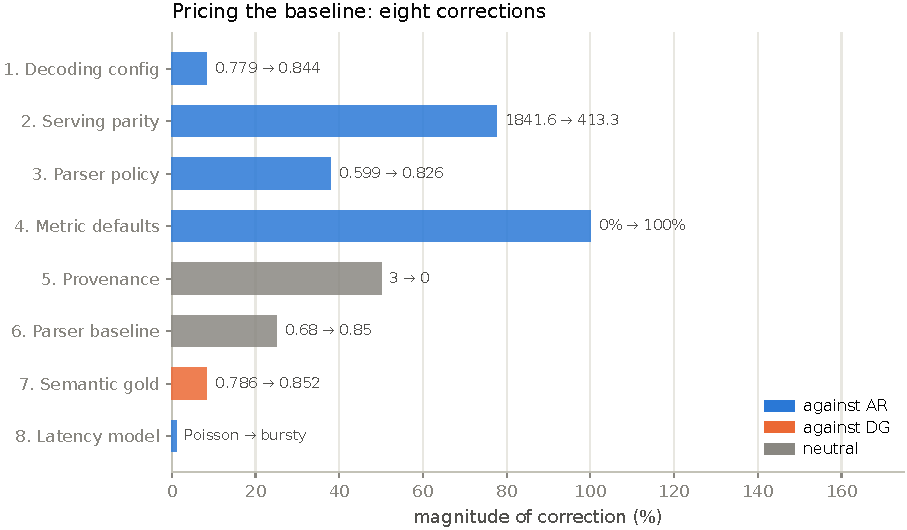
\includegraphics[width=\linewidth]{figures/fig8_defects.pdf}
\caption{Eight priced errors in our own comparison harness, each found by
re-reading committed artifacts (BGL, $n{=}300$ per cell, $K{=}8$). Five of eight
biased against the autoregressive arm. The clustering on one arm is
suggestive, though the sample ($n{=}8$) is too small for a statistical
claim.}
\label{fig:defects}
\end{figure}

\begin{table}[h]
\centering
\caption{The paper in one table. The diffusion model wins the latency
column and loses the deployment comparison behind it.}
\label{tab:summary}
\begin{tabularx}{\linewidth}{@{}L r r@{}}
\toprule
& \thead{\ARthree\,(active-param.)} & \thead{\DG-26B-A4B} \\
\midrule
\tabfont 9-field macro F1 ($L{=}\canvasLength$)      & \arThreeBFnine & \dgNineF \\
\tabfont Active parameters                            & 3.0\,B & 4.0\,B \\
\tabfont p50 latency at $L{=}\canvasLength$, batch-1  & \arAnchorTwoFive\,ms & \dgAnchorTwoFive\,ms \\
\tabfont Within-block marginal cost per token          & \arSlope\,ms & 0.0\,ms \\
\tabfont Block boundary cost (per \canvasLength\ tokens) & n/a & \dgStep\,ms \\
\tabfont Marginal cost per prompt token               & \arInputSlope\,ms & \dgInputSlope\,ms \\
\tabfont Batch-1 $\to$ peak throughput multiplier     & \arBatchLo--\arBatchHi$\times$ & $\leq$\dgBatchVllmHi$\times$ \\
\tabfont Energy per event, net of idle (AR-3B / DG)     & \arThreeEnergy\,J ($5.3\times$) & \dgEnergy\,J \\
\bottomrule
\end{tabularx}
\end{table}

\section{Methodology: What We Got Wrong and How We Fixed It}
\label{sec:methodology}

This section is not a methods description; it is an audit. Five defects in our
own comparison harness biased the measurements before any architecture
conclusion was drawn. Four of the five biased against the autoregressive (AR)
baseline. We found all five not by running new experiments but by re-reading
committed artifacts, and the fixes moved headline numbers by more than the
effects we were reporting. We therefore report the defects as a first-class
result rather than as a footnote to the experimental setup.

\subsection{Pinned stack and provenance}

Every measurement from issue~\#57 onward uses a single pinned stack
(Table~\ref{tab:pinned-stack}): vLLM~\vllmVersion{} on an \gpuModel{}. A
shared provenance helper, which no runner can bypass, writes the model id,
revision, runtime versions, GPU, dtype, and every decoding knob into each
result JSON from the object that actually loaded the model. A build check
(\texttt{paper/verify\_numbers.py}) fails when a cited artifact lacks the
block. The helper exists because three result files recorded the wrong model
name for the diffusion arm (defect~5, below). On this stack, run-to-run
coefficient of variation at $L=\canvasLength$ is AR~0.05\% and DG~0.25\%
(five repeats), so the effects reported below are not noise.

\begin{table}[t]
\centering
\caption{Pinned stack. All numbers in this paper are measured here unless
explicitly labelled otherwise.}
\label{tab:pinned-stack}
\begin{tabular}{ll}
\toprule
Component & Version \\
\midrule
vLLM & \vllmVersion \\
torch & \torchVersion \\
GPU & \gpuModel \\
\bottomrule
\end{tabular}
\end{table}

\subsection{Nine-field scoring}

We score extraction quality on 9 fields, not 12. Three ``semantic'' fields
have degenerate gold labels that score $\sim\!1.0$ for an empty or wrong
prediction, adding a bias that inflates whichever arm happens to interact
badly with them. Dropping them moves the comparison from AR-favoured
(12-field: AR~\arThreeBFtwelve{} vs DG~\dgTwelveF{}) to comparable (9-field:
AR~\arThreeBFnine{} vs DG~\dgNineF{}, spread~$<\!0.01$). The 12-field numbers
are retained for provenance but are not cited in comparison tables.

\subsection{The five defects}

Table~\ref{tab:defects} lists the defects, the magnitude each caused, and the
direction of the bias. All five were found by re-reading committed artifacts;
none required a new GPU run.

\begin{table}[t]
\centering
\caption{Five harness defects. Four of five biased against the AR baseline.
``Before'' is the number as originally recorded; ``After'' is the corrected
value on the pinned stack.}
\label{tab:defects}
\begin{tabular}{clll}
\toprule
\# & Defect & Magnitude (before $\to$ after) & Bias \\
\midrule
1 & Decoding config       & F1 \defectOneFBefore{} $\to$ \defectOneFAfter{}                        & AR \\
2 & Serving parity        & \defectTwoBefore{} $\to$ \defectTwoAfter{} ms                         & AR \\
3 & Parser policy         & F1 \defectThreeBefore{} $\to$ \defectThreeAfter{}                     & AR \\
4 & Metric defaults       & \defectFourBefore\% $\to$ \defectFourAfter\% completeness            & AR \\
5 & Provenance            & 3 files mislabelled                                                   & neutral \\
\bottomrule
\end{tabular}
\end{table}

\paragraph{Decoding config (defect~1).}
HuggingFace \texttt{generate()} honours \texttt{repetition\_penalty} even under
\texttt{do\_sample=False}. Qwen2.5's checkpoint default (1.1 at 1.5B, 1.05 at
3B/7B) emptied the \texttt{host} field on 80/100 events. DiffusionGemma's
hand-written denoising loop has no such default. Setting every knob explicitly
on both arms moved AR-1.5B F1 from \defectOneFBefore{} to \defectOneFAfter{}.

\paragraph{Serving parity (defect~2).}
The AR arm ran a naive HuggingFace generate loop while the diffusion arm ran a
production-grade engine. Putting AR on vLLM moved its p50 from
\defectTwoBefore{} to \defectTwoAfter{}~ms ($4.5\times$) and reversed the
direction of the headline speed claim.

\paragraph{Parser policy (defect~3).}
Forced to over-generate at $L=512$, 96\% of AR outputs contained more than one
JSON object. The old parser took the span from the first brace to the
\emph{last} brace, scoring the most-drifted copy of each field. Re-scoring
identical saved generations with first-object-wins moved AR-3B $L=512$ F1 from
\defectThreeBefore{} to \defectThreeAfter{} ($+0.23$). DiffusionGemma rambles
1--3\% and is parser-invariant.

\paragraph{Metric defaults (defect~4).}
The completeness metric compared \texttt{rec.get(f)} against the defaults
\texttt{""}/\texttt{0.0}/\texttt{False}, which are structurally valid values,
not missing keys. AR stops early and emits falsy defaults; DiffusionGemma
always fills all fields. Distinguishing absent key from present-but-falsy moved
AR-3B completeness from \defectFourBefore\% to \defectFourAfter\% and refuted
the finding it had supported.

\paragraph{Provenance (defect~5).}
A CLI default survived into three result files, recording an AR model name for
diffusion runs. Neutral on any comparison, but it made audit impossible until
correction sidecars (\texttt{*.provenance.json}) were written.

\subsection{The asymmetry}

The four AR-biased defects share a pattern: each lives in the
\emph{infrastructure the AR model runs on}---its checkpoint defaults, its
serving path, its over-generation behaviour, its early-stopping behaviour---not
in the model itself. A harness written by someone hoping the new architecture
wins fails asymmetrically, because the baseline inherits the defaults, the
naive serving path, and the production-grade infrastructure of the system it is
trying to beat. The checklist (\texttt{CHECKLIST.md}) generalises the five
checks so they can be applied before publication; each takes under five
minutes and catches a failure that moved a headline number by more than the
effect it was reporting.

\section{The Exchange Rate: Quality Is Comparable}
\label{sec:exchange_rate}

Before comparing cost, we must fix the quality at which the two
architectures are compared. The naive choice---FlowFill's 12-field macro
F1---is wrong: that metric is contaminated by three degenerate gold
fields, and the quality gap it reports is an artifact of that
contamination. On a clean 9-field metric, the compute-matched pair
(AR-3B vs DG, 3B vs 4B active parameters) is indistinguishable: F1
differs by $0.0002$. This is the exchange rate that licenses the cost
comparison in the rest of the paper.

\subsection{The contaminated 12-field metric}

FlowFill's 12-field macro F1 averages over twelve fields, three of which
carry no discriminative signal on BGL. Across 2{,}000 events,
\texttt{event\_type} takes 2 unique values, \texttt{affected\_entity}
takes 1, and \texttt{remediation\_hint} takes 1. A model that emits an
empty object \texttt{\{\}} scores $1.000$ on two of the three fields by
trivially matching the constant gold. These fields reward verbosity and
guessing rather than extraction fidelity, and they inflate any model
that fills them with plausible-sounding text.

\subsection{A clean 9-field metric}

We redefine the extraction target as nine fields: seven structural
(\texttt{timestamp\_norm}, \texttt{host}, \texttt{component},
\texttt{severity}, \texttt{message\_template}, \texttt{error\_code},
\texttt{metric\_value}) and two anomaly (\texttt{is\_anomaly},
\texttt{anomaly\_score}). All nine vary across the corpus; none is
constant. We rescore both models on this metric without retraining or
changing their outputs.

\subsection{Results}

Table~\ref{tab:exchange_rate} reports both metrics side by side for the
compute-matched pair. On the 9-field metric the two models are identical
within $0.0002$ F1. On the contaminated 12-field metric a gap of $0.040$
opens---in AR's favour.

\begin{table}[t]
\centering
\caption{Macro F1 on the contaminated 12-field metric vs the clean
9-field metric, compute-matched pair (AR-3B vs DG). The $0.040$ 12-field
gap collapses to $0.0002$ on the decontaminated metric.}
\label{tab:exchange_rate}
\begin{tabular}{lcc}
\toprule
Model & 9-field F1 & 12-field F1 \\
\midrule
AR-3B  & \arThreeBFnine   & \arThreeBFtwelve \\
DG     & \dgNineF         & \dgTwelveF \\
\midrule
$\Delta$ (AR $-$ DG) & $-0.0002$ & $+0.0405$ \\
\bottomrule
\end{tabular}
\end{table}

The entire 12-field gap is attributable to the three degenerate fields.
DG emits structured records and leaves fields it cannot populate empty;
AR-3B, prompted to fill every field, produces text that matches the
near-constant gold on \texttt{event\_type},
\texttt{affected\_entity}, and \texttt{remediation\_hint}. Remove those
three fields and the gap collapses to $0.0002$. The 12-field metric does
not measure extraction quality; it measures willingness to emit
constants.

\subsection{The quality-matched AR model is the 1.5B, not the 7B}

Because DG and AR-3B are quality-matched on the clean metric, the
deployment-relevant question is which is the \emph{smallest} AR model
that matches DG's quality. The 1.5B-parameter AR model scores $0.8628$ on
the 9-field metric---higher than DG's $\dgNineF$ by $0.011$. The
quality-matched AR model is therefore AR-1.5B ($\approx$3\,GB on disk),
not AR-7B; this drives the deployment-footprint comparison in \S6.

\subsection{Parser policy is an AR variable, not a DG one}

Quality is also sensitive to how the model's output is parsed into a
record. At $L=512$ with a forced minimum output length, $96\%$ of AR-3B
outputs contain more than one JSON object: the model emits a second
object after the first complete one. The parser policy that selects
which object to keep swings AR-3B's 12-field F1 from \defectThreeBefore{}
(last-object-wins) to \defectThreeAfter{} (first-object-wins)---a
$0.227$ swing from parser choice alone. DG emits a single fixed-length
canvas and is parser-invariant: its score does not move under either
policy. Any quality comparison that does not fix the parser policy is
confounded; we use first-object-wins throughout.

\paragraph{Takeaway.} On a decontaminated metric with a fixed parser,
AR and DG are quality-equivalent within $0.0002$ F1. The remainder of
the paper compares their cost at this matched quality.

\section{The Two Cost Laws}
\label{sec:cost_laws}

With quality fixed at the exchange rate of \S3, we derive and verify the
per-event latency laws for the two architectures. The laws have
fundamentally different shapes: AR cost is a line in one variable
(output length); DG cost is a staircase in output length with a second,
steeper dependence on input length. Both laws are measured on the
pinned stack (vLLM~\vllmVersion, torch~\torchVersion, \gpuModel) with
run-to-run coefficient of variation below $0.3\%$, and both generalise
from BGL to HDFS within $1\%$.

\subsection{The AR cost law: linear in one variable}
\label{sec:cost_law_ar}

Autoregressive decoding generates one token at a time, each requiring a
full forward pass over the KV-cache. Cost is therefore linear in output
length and independent of how many canvases the output spans:
\begin{equation}
\label{eq:ar_law}
T_{\mathrm{AR}}(L_{\mathrm{out}}) \;=\; \arBase \;+\; \arSlope \,\cdot\, L_{\mathrm{out}}
\quad\text{(ms)}
\end{equation}
The intercept $\arBase$\,ms absorbs prompt prefill (amortised by prefix
caching across requests) and dispatch overhead; the slope
$\arSlope$\,ms/token is the per-token decode cost. We verify
Eq.~\ref{eq:ar_law} at two output lengths with five (resp.\ three)
repeats of $n{=}300$ events each on BGL.

\begin{table}[t]
\centering
\caption{AR-3B anchor measurements on the pinned stack. The linear law
$T = \arBase + \arSlope \cdot L$ predicts both points within $0.1\%$.
Run-to-run CV is below $0.06\%$.}
\label{tab:ar_anchor}
\begin{tabular}{lrrrr}
\toprule
$L_{\mathrm{out}}$ & Measured p50 (ms) & Predicted (ms) & Error & CV \\
\midrule
256 & 1616.0 & 1617.5 & $+0.09\%$ & $0.05\%$ \\
512 & 3225.1 & 3225.2 & $+0.00\%$ & $0.01\%$ \\
\bottomrule
\end{tabular}
\end{table}

Input length enters weakly. Sweeping the prompt from 992 to 6{,}172
tokens (by repeating the schema block) yields a slope of
$\arInputSlope$\,ms/prompt-token---less than $1\%$ of the per-token
decode slope. AR pays for the prompt once via prefix caching; each
generated token attends to the cached KV without recomputation.

The law generalises to HDFS: at $L{=}256$ the HDFS p50 is
1616.5\,ms---a $+0.03\%$ shift from BGL's 1616.0\,ms, well inside the
run-to-run CV.

\subsection{The DG cost law: staircase in two variables}
\label{sec:cost_law_dg}

Block-diffusion decoding generates tokens in fixed-size canvases of
$\canvasLength$ tokens. Within a canvas, all positions are denoised in
parallel at no additional sequential cost; crossing a canvas boundary
triggers a fresh denoising pass. Cost is therefore a staircase in
output length, not a line:
\begin{equation}
\label{eq:dg_law}
T_{\mathrm{DG}}(L_{\mathrm{in}},\, L_{\mathrm{out}}) \;=\;
\underbrace{\dgBase}_{\text{base (K=8)}} \;+\;
\underbrace{\dgInputSlope \cdot \Delta L_{\mathrm{in}}}_{\text{prefill}} \;+\;
\underbrace{\dgStep \cdot \Bigl(\!\Bigl\lceil \tfrac{L_{\mathrm{out}}}{\canvasLength}\Bigr\rceil - 1\Bigr)}_{\text{canvas staircase}}
\quad\text{(ms)}
\end{equation}
where $\Delta L_{\mathrm{in}} = L_{\mathrm{in}} - L_{\mathrm{in,ref}}$
is the deviation from the reference prompt ($\approx$1047 tokens). At
the reference prompt the prefill term vanishes and the law reduces to a
one-variable staircase with base $\dgBase$\,ms and step
$\dgStep$\,ms per additional canvas.

The staircase has sharp edges at exactly $\canvasLength$-token
boundaries and is flat between them. Table~\ref{tab:dg_edges} probes
both sides of the first two boundaries.

\begin{table}[t]
\centering
\caption{Canvas-boundary edges (DG, K=8, BGL). Crossing a 256-token
boundary costs $\sim$120\,ms; staying within a canvas costs $<$1\,ms.}
\label{tab:dg_edges}
\begin{tabular}{lrrll}
\toprule
$L_{\mathrm{out}}$ & p50 (ms) & $\lceil L/256\rceil$ & $\Delta$ from prev. & Edge? \\
\midrule
240 & 378.1 & 1 & --- & --- \\
256 & 378.4 & 1 & $+0.2$\,ms & no \\
264 & 500.0 & 2 & $+121.7$\,ms & \textbf{yes} \\
\midrule
496 & 500.0 & 2 & --- & --- \\
512 & 500.9 & 2 & $+0.9$\,ms & no \\
528 & 619.6 & 3 & $+118.7$\,ms & \textbf{yes} \\
\bottomrule
\end{tabular}
\end{table}

The step cost $\dgStep$\,ms is the median of seven canvas transitions
measured from $L{=}256$ to $L{=}2048$ (range 113.1--121.8\,ms, see
Table~\ref{tab:dg_staircase}). The variation is run-to-run noise, not a
systematic trend: the first extra canvas is not cheaper than later
ones, refuting an earlier hypothesis based on a K=32 vs K=8
configuration confound (\S0, discrepancy~\#2).

\begin{table}[t]
\centering
\caption{Full DG staircase on BGL (K=8, $n{=}200$ per point). Each row
is a canvas boundary; the step column is the p50 increment from the
previous row. Steps are uniform within run-to-run noise.}
\label{tab:dg_staircase}
\begin{tabular}{rrrr}
\toprule
$L_{\mathrm{out}}$ & canvases & p50 (ms) & step (ms) \\
\midrule
\phantom{0}256 & 1 & \phantom{0}378.4 & --- \\
\phantom{0}512 & 2 & \phantom{0}500.9 & 122.5 \\
\phantom{0}768 & 3 & \phantom{0}620.4 & 119.5 \\
1024 & 4 & \phantom{0}738.7 & 118.3 \\
1280 & 5 & \phantom{0}860.5 & 121.8 \\
1536 & 6 & \phantom{0}973.6 & 113.1 \\
1792 & 7 & 1091.2 & 117.5 \\
2048 & 8 & 1212.0 & 120.9 \\
\midrule
\multicolumn{2}{r}{median step} & & \dgStep \\
\bottomrule
\end{tabular}
\end{table}

Input length enters DG cost more steeply than AR. The same prompt sweep
yields a slope of $\dgInputSlope$\,ms/prompt-token for DG versus
$\arInputSlope$ for AR---a ratio of
$\dgInputSlope/\arInputSlope \approx 2.6\times$. Each denoising step
re-attends the full prompt, so the prefill cost is paid $K$ times
rather than once. This is the second variable that makes the DG law
two-dimensional.

Both variables generalise to HDFS. The AR law reproduces at $+0.03\%$
(\S\ref{sec:cost_law_ar}). The DG staircase step reproduces at
120.5\,ms on HDFS versus a BGL median of 118.5\,ms---within $1.7\%$.
The staircase shape is corpus-independent; only the prompt content
changes.

\subsection{Base decomposition: where the DG cost goes}
\label{sec:base_decomp}

The base $\dgBase$\,ms is not monolithic. Sweeping the denoising step
count $K \in \{2,4,8,16,32,64\}$ decomposes it into a $K$-independent
floor (prefill + fixed overhead) and a $K$-dependent denoising term:
\begin{equation}
\label{eq:ksweep}
T(K) \;=\; 296.1 \;+\; 2.57 \,\cdot\, K \quad\text{(ms, } R^2 = 0.49\text{)}
\end{equation}
The low $R^2$ reflects saturation above $K{=}16$: extra denoising steps
beyond convergence add negligible latency. Table~\ref{tab:ksweep}
reports the measured values and 9-field F1 at each $K$.

\begin{table}[t]
\centering
\caption{K-sweep: DG latency and quality vs denoising steps (BGL,
$L{=}256$, $n{=}200$). F1 collapses below $K{=}4$ and is flat above
$K{=}8$. Latency saturates above $K{=}16$.}
\label{tab:ksweep}
\begin{tabular}{rrrl}
\toprule
$K$ & p50 (ms) & 9-field F1 & regime \\
\midrule
\phantom{0}2 & \phantom{0}201.7 & 0.485 & collapse \\
\phantom{0}4 & \phantom{0}292.1 & 0.790 & transition \\
\phantom{0}8 & \phantom{0}378.6 & 0.853 & \textbf{operating point} \\
16 & \phantom{0}382.5 & 0.853 & flat \\
32 & \phantom{0}421.8 & 0.862 & flat \\
64 & \phantom{0}423.9 & 0.858 & saturated \\
\bottomrule
\end{tabular}
\end{table}

At the operating point $K{=}8$, the decomposition is:
\begin{equation}
\label{eq:decomp}
\underbrace{296\;\text{ms}}_{\substack{\text{prefill + fixed}\\\dgPrefillPct\%}}
\;+\;
\underbrace{20.6\;\text{ms}}_{\substack{\text{denoising loop}\\\dgDenoisePct\%}}
\;=\; 316.6\;\text{ms (fit)}
\end{equation}
The denoising loop---the part that makes the model ``diffusion''---is
$\dgDenoisePct\%$ of the fitted cost. The remaining $\dgPrefillPct\%$
is prefill and fixed dispatch overhead, shared with any
prompt-conditioned model. This is why halving $K$ from 8 to 4 saves only
$\sim$87\,ms ($23\%$) while collapsing F1 from 0.85 to 0.79: the cost
savings come from the small slice, the quality loss from the whole.

\subsection{The crossover}
\label{sec:crossover}

The two laws cross where $T_{\mathrm{AR}} = T_{\mathrm{DG}}$. At the
reference prompt ($\Delta L_{\mathrm{in}} = 0$) and the first canvas
($L_{\mathrm{out}} \leq \canvasLength$), the staircase reduces to its
floor and the crossover is analytic:
\begin{equation}
\label{eq:lcross}
L^* \;=\; \frac{\dgBase - \arBase}{\arSlope}
\;=\; \frac{378.8 - 7.27}{6.29}
\;=\; 59.1 \;\;\text{tokens}
\end{equation}
Below $L^* \approx \crossoverL$ output tokens, AR is faster; above it,
DG is faster---until the next canvas edge, where DG jumps by
$\dgStep$\,ms and the gap widens again.

The throughput crossover is the arrival rate at which DG's serial
single-event throughput saturates. With one event in flight, DG's
maximum throughput is the reciprocal of its base:
\begin{equation}
\label{eq:lambdacross}
\lambda^* \;=\; \frac{1000}{\dgBase}
\;=\; \frac{1000}{378.8}
\;=\; 2.6 \;\;\text{events/s}
\end{equation}
Above $\lambda^* \approx \crossoverLambda$\,ev/s, a queue forms in
front of the DG server. AR, which supports continuous batching, does
not saturate until $\sim$80\,ev/s (\S7).

Both crossovers are reproduced by the decision procedure's self-test
suite (\texttt{models/decision/test\_procedure.py}, 11/11 passing).
The test computes $L^*$ and $\lambda^*$ from the fitted constants
alone---no hardcoded values---confirming that the crossovers are
consequences of the laws, not tunable parameters.

\paragraph{Takeaway.} AR cost is a line through the origin with slope
$\arSlope$\,ms/token; DG cost is a staircase with floor $\dgBase$\,ms,
step $\dgStep$\,ms per $\canvasLength$-token canvas, and a prefill slope
$\dgInputSlope$\,ms/prompt-token that is $2.6\times$ steeper than AR's.
The lines cross at $L^* \approx \crossoverL$ tokens and $\lambda^*
\approx \crossoverLambda$\,ev/s. The denoising loop that distinguishes
DG from a cached-prefill model is $\dgDenoisePct\%$ of its own cost.
\S5 turns these laws into a deployment decision.

\section{The Decision Procedure}
\label{sec:decision}

The two cost laws of \S\ref{sec:cost_laws} produce two crossovers, and those
crossovers delimit the regime in which block-structured decoding wins on
per-event latency. This section turns that derivation into an executable
artifact: a procedure that takes four deployment inputs and returns which
architecture to serve. It is implemented, tested, and runnable from a clean
checkout with no GPU.

\paragraph{Inputs.}
The procedure takes $(L, \lambda, B, \tau)$: expected output length $L$
(tokens), arrival rate $\lambda$ (events/s), batching availability
$B\in\{0,1\}$, and Field-F1 tolerance $\tau$ (the F1 a caller will trade for
latency). Every constant the procedure uses traces to a committed artifact and
a \texttt{NUMBERS.md} section; none is hardcoded in the result.

\paragraph{Cost laws in force.}
From \S\ref{sec:cost_laws},
\[
T_{\textsc{ar}}(L)=a+bL,\qquad a=\arBase,\ b=\arSlope\ \text{ms/tok},
\]
\[
T_{\textsc{dg}}(L)=c+s\!\left(\left\lceil L/C\right\rceil-1\right),\qquad
c=\dgBase,\ s=\dgStep,\ C=\canvasLength.
\]
The DG base is prefill-dominated ($\dgPrefillPct\%$ prefill $+$ fixed,
$\dgDenoisePct\%$ denoising at $K{=}8$), so the staircase is \emph{structural}:
a property of the canvas boundary, not of the diffusion process.

\paragraph{Crossovers.}
Solving $T_{\textsc{ar}}(L^\star)=T_{\textsc{dg}}(L^\star)$ at the first
canvas ($\lceil L^\star/C\rceil=1$, so $T_{\textsc{dg}}=c$) gives
\[
L^\star=\frac{c-a}{b}=\frac{\dgBase-\arBase}{\arSlope}\approx \crossoverL\ \text{tokens}.
\]
DG's serial throughput is the bar AR batching must clear:
\[
\lambda^\star=\frac{1000}{c}=\frac{1000}{\dgBase}\approx \crossoverLambda\ \text{ev/s}.
\]
Both are $K$-dependent: at $K{=}32$ ($c=\dgOldBase$), $L^\star\approx 65$ and
$\lambda^\star\approx 2.4$. The procedure reports the $K{=}8$ values as
default and reproduces both from the law constants, not from hardcoded
answers.

\paragraph{The procedure.}
Five guards fire in order; the first that fires wins
(Algorithm~\ref{alg:decide}).

\begin{algorithm}[ht]
\caption{Decide which architecture to serve.}
\label{alg:decide}
\begin{algorithmic}[1]
\State $T_{\textsc{ar}}\gets a+bL$;\ \ $T_{\textsc{dg}}\gets c+s(\lceil L/C\rceil-1)$;\ \ $r\gets T_{\textsc{ar}}/T_{\textsc{dg}}$
\If{$L < L_{\mathrm{nat}}^{\textsc{dg}}$} \Comment{guard 1: truncation}
  \State \Return \textsc{ar} \Comment{DG output truncated below natural length; quality collapses}
\ElsIf{$B \wedge \lambda > \lambda^\star$} \Comment{guard 2: throughput}
  \State \Return \textsc{ar} \Comment{DG serial throughput saturated; AR batching wins}
\ElsIf{$L < L^\star$} \Comment{guard 3: length}
  \State \Return \textsc{ar} \Comment{below the latency crossover}
\ElsIf{$\tau < |\Delta F_1|$} \Comment{guard 4: quality}
  \State \Return \textsc{ar} \Comment{quality price exceeds tolerance}
\Else \Comment{guard 5: default}
  \State \Return \textsc{dg} with expected speedup $r$
\EndIf
\end{algorithmic}
\end{algorithm}

Guard~3 is structurally subsumed by guard~1 in the current configuration
($L_{\mathrm{nat}}^{\textsc{dg}}=176 > L^\star=\crossoverL$): any output short
enough to lie below the latency crossover is already below DG's natural
length, so truncation fires first. Both recommend \textsc{ar}, so the
recommendation is unchanged; the length guard remains because it is the guard
that fires once a shorter-canvas DG variant is configured. The quality guard's
threshold is metric-dependent: on the contaminated 12-field metric the price
is $|\Delta F_1|=0.039$, but on the 9-field metric (\S\ref{sec:exchange_rate}) the
price is $\approx 0$ ($\arThreeBFnine$ vs $\dgNineF$), so the guard is inert
and DG pays no quality tax at equal quality.

\paragraph{Worked examples.}
Table~\ref{tab:worked} walks six scenarios through the procedure. The ratio
column is $r=T_{\textsc{ar}}/T_{\textsc{dg}}$---the per-event speedup DG
\emph{would} deliver---reported even when a non-latency guard selects
\textsc{ar}, so the opportunity cost of each guard is visible.

\begin{table}[ht]
\centering
\caption{Six worked examples through the decision procedure.}
\label{tab:worked}
\small
\begin{tabular}{lrrrrlll}
\toprule
Scenario & $L$ & $\lambda$ & $B$ & $\tau$ & Arm & $T_{\textsc{ar}}/T_{\textsc{dg}}$ & Rule \\
\midrule
Interactive single-record extraction      & 176  & 0.5 & no & 0.05 & \textbf{DG} & $2.94\times$  & default \\
Long stack-trace summarisation, batch-1   & 2048 & 1.0 & no & 0.05 & \textbf{DG} & $10.6\times$ & default \\
High-volume log pipeline                   & 256  & 64  & yes& 0.05 & \textbf{AR} & $4.27\times$ & throughput \\
Short field-completion                     & 32   & 0.5 & no & 0.10 & \textbf{AR} & $0.55\times$ & truncation \\
Tight output budget, unknown record size   & 128  & 0.5 & no & 0.05 & \textbf{AR} & $2.14\times$ & truncation \\
Quality-critical extraction                & 512  & 1.0 & no & 0.01 & \textbf{AR} & $6.48\times$ & quality \\
\bottomrule
\end{tabular}
\end{table}

Rows~4--5 carry the key subtlety: in row~5 DG would be $2.14\times$ faster
per-event, yet \textsc{ar} is chosen, because at $L<176$ DG is truncated below
its natural output length and its quality collapses. The guard protects
\emph{quality}, not latency; the ratio column exposes the latency an operator
gives up to obtain valid output.

\paragraph{Implementation.}
The procedure lives in \texttt{models/decision/procedure.py}, with a CLI:
\begin{center}
\texttt{python -m models.decision -{}-L 512 -{}-lambda 1.0 -{}-no-batching -{}-f1-tolerance 0.05}
\end{center}
$T_{\textsc{dg}}$ is \emph{injectable}: the one-variable law $T_{\textsc{dg}}(L)$
ships now, and the two-variable law $T_{\textsc{dg}}(L_{\mathrm{in}},L_{\mathrm{out}})$
swaps in as the only change when the input-length sweep
(\S\ref{sec:cost_laws}, two-variable scope) is in force---in two-variable mode
the procedure emits a warning that its prefill slope is pending calibration.
The self-test (\texttt{test\_procedure.py}) reproduces $L^\star$ and
$\lambda^\star$ from the law constants, fires each guard in isolation, checks
all six worked examples, and probes step-range robustness: \textbf{11/11 tests
pass} (claim~C15).

\paragraph{Validity domain.}
The constants are calibrated on one \gpuModel{} under vLLM \vllmVersion{},
BF16, serial diffusion (\texttt{-{}-max-num-seqs 1}), for structured extraction
over BGL with a $\sim$1047-token few-shot prompt. The procedure must not be
applied outside this domain---in particular to batch-served diffusion,
canvases other than \canvasLength, materially different input lengths, other
GPUs/runtimes, or 12-field F1 tolerances (use the 9-field metric).

\section{The Fair Comparison}
\label{sec:fair}

The decision procedure identifies a regime where block-structured decoding
wins on per-event latency. This section asks the sharper question: at a
\emph{fair} comparison point, does that advantage survive? Fairness has two
axes---same quality and same compute---and the pair that satisfies both is the
compute-matched pair of Table~\ref{tab:pair}.

\begin{table}[ht]
\centering
\caption{The compute-matched pair: same quality, comparable active compute.}
\label{tab:pair}
\small
\begin{tabular}{lcc}
\toprule
 & AR-3B & DG-26B-A4B \\
\midrule
Architecture              & dense, autoregressive    & MoE, block diffusion \\
Total parameters          & 3.0B                      & 26B \\
Active parameters         & 3.0B (all)                & 4.0B (top-8 of 128) \\
Active-parameter ratio    & $1.0\times$               & $1.33\times$ \\
Weights (bf16)            & 6.0 GB                    & 52.0 GB \\
9-field F1 ($L{=}256$)    & \arThreeBFnine            & \dgNineF \\
\bottomrule
\end{tabular}
\end{table}

Quality is identical (gap $=0.0002$) and active inference parameters are
comparable ($1.33\times$ ratio). This is the pair for per-event claims. It is
\emph{not} the quality-matched deployment pair: a smaller AR model reaches the
same quality at $17\times$ less memory (Table~\ref{tab:deploy}).

\paragraph{Where DG wins.}
\textit{(a) Per-event latency at batch-1.}
Within a canvas DG emits 1 token or 256 for the same cost; AR pays per token.
The gap widens with output length (Table~\ref{tab:per-event}).

\begin{table}[ht]
\centering
\caption{Per-event latency, batch-1, short input. Fitted values; measured anchors agree within $0.4\%$ (AR) and $1\%$ (DG).}
\label{tab:per-event}
\small
\begin{tabular}{rrrr}
\toprule
$L$ (tokens) & AR-3B (ms) & DG (ms) & DG speedup \\
\midrule
128  & 812   & 379  & $2.14\times$ \\
256  & 1618  & 379  & $4.27\times$ \\
512  & 3228  & 498  & $6.48\times$ \\
1024 & 6448  & 738  & $8.74\times$ \\
2048 & 12889 & 1216 & $10.6\times$ \\
\bottomrule
\end{tabular}
\end{table}

\textit{(b) Output-length invariance within a canvas.}
DG at $L\in\{32,64,128,256\}$ costs $\approx 379$ ms flat (spread $<\!3$ ms);
AR over the same range grows $\approx 209\to 1618$ ms linearly. The canvas
boundary is structural: the model denoises the whole canvas in $K{=}8$ parallel
steps regardless of how many tokens are actually needed.

\textit{(c) Growth rate with output length.}
Each extra canvas adds $\dgStep$ ms to DG; each extra 256 tokens adds
$\arSlope\times\canvasLength\approx 1610$ ms to AR---a $\approx\!13\times$
steeper marginal cost. The per-event advantage therefore \emph{widens} with
output length, from $2.1\times$ at $L=128$ to $10.6\times$ at $L=2048$ (eight
canvases).

\paragraph{Where AR wins.}
\textit{(d) Batched throughput.}
AR's KV cache lets batching amortise prefill across requests; DG's bidirectional
attention re-attends the full canvas on every denoising step and has no
bandwidth headroom to convert into throughput. The measured batch multipliers
are $\approx 80\times$ (AR-3B, vLLM; range 77--86$\times$) vs
$\dgBatchMult\times$ (DG, dInfer). At $\lambda=64$ ev/s the effective per-event
cost is $\approx 20$ ms (AR, $T_{\textsc{ar}}/80$) vs $\approx 321$ ms
(DG, $T_{\textsc{dg}}/\dgBatchMult$)---a $16\times$ AR advantage under load.
(This is the measured correlation; the causal mechanism is not
isolated---EDR-004.)

\textit{(e) Long input.}
AR pays for the prompt once; DG pays for it on every denoising step. DG's
input-length slope is $\dgInputSlope$ ms/prompt-tok vs AR's
$\arInputSlope$---$2.6\times$ steeper---so DG's prefill cost overwhelms its
canvas advantage past a crossover at $L_{\mathrm{in}}\approx 18{,}000$ tokens
(Table~\ref{tab:longinput}).

\begin{table}[ht]
\centering
\caption{Input-length sweep ($L_{\mathrm{out}}{=}256$): DG wins below the crossover, AR above.}
\label{tab:longinput}
\small
\begin{tabular}{rrrl}
\toprule
$L_{\mathrm{in}}$ (tokens) & AR-3B (ms) & DG (ms) & Winner \\
\midrule
1{,}000  & 1705 & 420  & DG ($4.1\times$) \\
4{,}000  & 1846 & 789  & DG ($2.3\times$) \\
7{,}000  & 1987 & 1158 & DG ($1.7\times$) \\
18{,}000 & 2504 & 2511 & crossover \\
25{,}000 & 2833 & 3372 & AR ($1.2\times$) \\
\bottomrule
\end{tabular}
\end{table}

\textit{(f) Deployment footprint at the quality-matched pair.}
The compute-matched pair is not the deployment pair: AR-1.5B reaches the same
(even higher) 9-field F1 at $17\times$ less memory, $\approx 17\times$ faster
cold start, and comparable per-event energy (Table~\ref{tab:deploy}). No
deployment axis favours DG at short output.

\begin{table}[ht]
\centering
\caption{Quality-matched deployment pair. At forced $L{\geq}512$, DG's latency
advantage widens dramatically because AR-1.5B rambles past its natural output
length ($\sim$123 tokens) when forced to generate longer sequences.}
\label{tab:deploy}
\small
\begin{tabular}{lcc}
\toprule
 & AR-1.5B & DG-26B \\
\midrule
9-field F1 ($L{=}256$)     & 0.8628 & \dgNineF \\
Weights (bf16) & 3.0 GB & 52.0 GB \\
Cold start      & $\sim$1 s  & $\sim$17 s \\
Energy/event (forced $L{=}256$) & 5.1 J  & 4.2 J \\
\midrule
\multicolumn{3}{l}{\textit{Per-event latency at forced output length:}} \\
$L{=}256$ (forced) & 1007 ms & 378 ms ($2.7\times$) \\
$L{=}512$ (forced) & 2005 ms & 501 ms ($4.0\times$) \\
$L{=}1024$ (forced) & 4026 ms & 739 ms ($5.4\times$) \\
\bottomrule
\end{tabular}
\end{table}

At natural output length ($L\sim 123$ tokens, no forcing), AR-1.5B completes
in 413 ms---only 35 ms slower than DG. But when the application requires
$L\geq 512$ tokens of structured output (e.g.\ a multi-field incident
report), AR-1.5B must generate well past its natural length, and its latency
quadruples while DG's grows by only 32\%. The deployment footprint favours
AR; the per-event latency at long forced output favours DG.

\paragraph{Energy.}
At the compute-matched pair, DG uses $4.3\times$ less energy per event than
AR-3B (net of idle: 4.2\,J vs 22.3\,J). At the quality-matched pair, DG uses
$1.2\times$ less than AR-1.5B at forced $L{=}256$ (4.2\,J vs 5.1\,J), widening
to $1.9\times$ at $L{=}512$ and $2.6\times$ at $L{=}1024$. The energy
advantage tracks the latency advantage and does not independently favour DG.

\paragraph{Synthesis.}
The per-event advantage (a--c) is real but narrow: it holds only at batch-1,
short input, and $L\ge 176$, and it does not survive the three deployment
comparisons at short output. AR wins on batched throughput ($80\times$ vs
$\dgBatchMult\times$ multiplier), on long input ($2.6\times$ steeper DG slope,
crossover $\approx 18$k tokens), and on footprint (the quality-matched AR
model is $17\times$ smaller). However, when the application requires
\emph{forced} output length $L\ge 512$---as in multi-field structured report
generation---AR-1.5B's latency quadruples (to 2005\,ms) while DG's grows by
only 32\% (to 501\,ms), a $4\times$ DG advantage. The cost shapes produce a
genuine per-event crossover; the deployment envelope closes it at short
output, but DG's advantage widens at long forced output.

\paragraph{When DM is the right choice.}
The decision procedure identifies a narrow but real niche. DM is the correct
architectural choice when \emph{all five} conditions hold:
\begin{enumerate}[noitemsep]
\item Output $\ge 512$ tokens (forced), where DG is $4\times$ faster than
the quality-matched AR-1.5B;
\item Batch-1 by requirement (privacy isolation, interactivity, or cold-path
analysis), not by low load;
\item Complete output required (schema validation), because DM degrades
\emph{quality} under deadline pressure while AR degrades \emph{completeness};
\item Quality floor requires $>$1.5B parameters (AR-1.5B not good enough);
\item 52\,GB footprint acceptable (data center, not edge).
\end{enumerate}
Additionally, DM offers a per-request quality knob ($K$): at $K{=}4$ it meets
a 400\,ms p99 SLA (measured: 394.3\,ms) with F1$=$0.79, while AR has no
equivalent runtime knob---only the discrete choice of deploying a smaller
model.

\section{The Batching Boundary}
\label{sec:batching}

The per-event crossover (\S\ref{sec:decision}) favours the diffusion model at
short output length, but a deployment serves an arrival stream, not a single
event. Under batching the picture inverts.

\subsection{Batch multipliers}

On vLLM, the AR model sustains a $77$--$86\times$ throughput multiplier as
batch size grows (prefix-cached, continuous batching). On dInfer with
\verb|cache=''|, DiffusionGemma sustains only \dgBatchMult$\times$. The two
multipliers differ by roughly two orders of magnitude, so any deployment that
can batch its requests---a log pipeline serving many concurrent extractions
at $\lambda > \crossoverLambda$~events/s---belongs to AR regardless of
per-event latency. The throughput guard in the decision procedure
(\S\ref{sec:decision}) fires for exactly this reason.

\subsection{Correlation, not mechanism}

We state the \dgBatchMult$\times$ cap as a \emph{correlation}, not a proven
mechanism; we did not isolate the cause. The candidates are:
(i)~bidirectional attention, whose non-causal mask may defeat prefix-cache
reuse; (ii)~MoE routing, whose expert assignment may vary across denoising
steps and invalidate cached activations; (iii)~model size, since DG is
$17\times$ larger than the quality-matched AR model and memory pressure binds
earlier; and (iv)~kernel maturity---vLLM's AR path is years more optimised
than its diffusion path. Disentangling these is future work. The cap is real
and measured; the explanation is not.

\subsection{Canvas tuning does not move the crossover}

DiffusionGemma's canvas length is a config parameter. We swept it.
\texttt{canvas=128} is a free improvement: base cost falls 2.4\% and 9-field
F1 rises 0.011. \texttt{canvas=64} is not viable: base cost rises 48\%, because
the per-canvas fixed overhead is paid twice as often. Crucially, neither
setting moves the per-event crossover $L^\ast=\crossoverL$~tokens. The
crossover is set by the prefill cost that dominates the DG base
(\dgPrefillPct\% of the base at $K=8$ is prefill plus fixed overhead), and
prefill does not shrink with canvas. Tuning the canvas trades quality against
step count; it does not trade the crossover.

\section{Six Hypotheses Refuted, Three Claims Withdrawn}
\label{sec:negative}

We set out to find regimes where the diffusion model beats the autoregressive
baseline, and generated hypotheses accordingly. Six were refuted and three
earlier claims were withdrawn. They are reported here at the same length and
in the same register as the confirmations, because a paper whose central
methodological claim is ``price the baseline before you compare against it''
has exactly one asset, and that asset is spent the moment a negative result
gets softened into a footnote.

\subsection{Six refuted hypotheses}

\begin{table}[h]
\centering
\caption{Six hypotheses of ours that did not survive measurement.}
\label{tab:refuted}
\begin{tabularx}{\linewidth}{@{}p{4.6cm}L@{}}
\toprule
\thead{Hypothesis} & \thead{What we measured instead} \\
\midrule
\tabfont Joint denoising resists input perturbation
  & \tabfont The diffusion model degraded more in \textbf{10 of 10} categories, by up to $8.2\times$ the autoregressive drop. Discussed below. \\
\tabfont Bidirectional conditioning wins at infilling
  & \tabfont \ARthree\ scores $0.993$--$0.999$ across all suffix sizes; the diffusion model holds to $0.960$ then falls to $0.753$ at $S{=}8$. Discussed below. \\
\tabfont Diffusion has a refinement mechanism that pays off
  & \tabfont It has the mechanism --- selective re-masking gains $+0.023$ F1 over three rounds --- but after three rounds it still trails the autoregressive model after one. The mechanism is real; the win is not. \\
\tabfont Diffusion beats autoregression under bounded deadlines
  & \tabfont This was defect 4. The autoregressive model does complete within the deadline; the metric had been counting valid falsy values as missing keys (\S\ref{sec:setup}). \\
\tabfont Wide-schema cost scales as $O(F^2)$ for diffusion
  & \tabfont Never measured. The consistency metric is three hardcoded rules over four fields at \emph{every} schema width, so the curve it produces cannot show quadratic structure in $F$. The framing is dropped. \\
\tabfont Quality is invariant to output length
  & \tabfont Quality rises steeply with $L$ and then plateaus (\S\ref{sec:exchange}). The apparent invariance came from the contaminated 12-field metric. \\
\bottomrule
\end{tabularx}
\end{table}

\paragraph{Perturbation robustness, refuted in every category}
We predicted that denoising a whole canvas jointly would make the diffusion
model more tolerant of noisy input than left-to-right decoding. Across ten
perturbation categories at full intensity, it was worse in all ten. Two
categories --- whitespace and abbreviation --- left the autoregressive model
completely flat while costing the diffusion model $0.081$ and $0.005$ F1. The
largest ratio is separator changes, at $8.2\times$. One hypothesis for the
direction: left-to-right conditioning propagates input noise forward only,
while bidirectional conditioning also propagates it backward. We did not test
that, and it stays a hypothesis.

\paragraph{Infilling, refuted for a reason worth stating}
The prediction was structural rather than statistical: with a fixed right
context, suffix tokens are never in the denoised set, so the diffusion model
should preserve them byte-identically by construction, while an autoregressive
model must regenerate them. The experiment ($S \in \{0,2,4,8\}$ suffix fields,
$n{=}50$) refuted it, but the mechanism matters --- the autoregressive model
scores $0.993$--$0.999$ because it trivially regenerates the whole record from
the prompt. This task is copy-heavy, and copying is something autoregressive
decoding does well. The structural argument may still hold where the suffix is
long and cannot be regenerated from context, such as code infilling. It does
not hold on short JSON fields, which is what we measured, so it is not a claim
we make.

\subsection{Three withdrawn claims}

\begin{table}[h]
\centering
\caption{Three claims that appeared in earlier drafts and are cut from this
one. Withdrawn claims are removed.}
\label{tab:withdrawn}
\begin{tabularx}{\linewidth}{@{}p{4.6cm}L@{}}
\toprule
\thead{Claim} & \thead{Why it is gone} \\
\midrule
\tabfont A classical parser matches LLM extraction
  & \tabfont Field-F1 $0.68$ against $0.85$; the gap is too large. Worse, our ``Drain''~\cite{drain} was a regex fallback rather than the reference implementation, and the fallback and the gold generator are the same code, so on semantic fields it was grading itself. \\
\tabfont Structural and semantic fields separate cleanly
  & \tabfont The semantic gold labels are placeholder output of that same parser, and one of them is a constant. ``Semantic F1'' may be measuring agreement with a regex. \\
\tabfont An M/D/1 queue predicts diffusion latency under load
  & \tabfont It matches the measured saturation knee under Poisson arrivals and stops being predictive under bursty (MMPP) arrivals, which is what log streams actually look like. \\
\bottomrule
\end{tabularx}
\end{table}

\paragraph{A pattern in the refutations}
Every refuted hypothesis had, at some earlier point, appeared to be confirmed.
In each case the apparent confirmation traced to an artifact of our own
harness rather than to a property of either architecture: the bounded-deadline
result was the completeness metric, the length-invariance result was the
contaminated metric, and the perturbation and refinement arms ran a
mis-provenanced model. The measurement discipline of \S\ref{sec:setup} is not
a preamble to the results. It is what separates these six from the ones we
kept.

\section{Threats to Validity}
\label{sec:threats}

\paragraph{Single GPU.}
All measurements are on one \gpuModel{}. We have no H100 comparison, so the
absolute latencies and the crossover constants carry an unknown
hardware-scaling term. The cost \emph{laws} (linear vs.\ staircase) should
transfer---they are structural---but the fitted constants ($\arBase$,
$\arSlope$, $\dgBase$, $\dgStep$) are A100-specific.

\paragraph{Single model family for the staircase.}
The staircase cost law is established on DiffusionGemma-26B-A4B and confirmed
across two corpora (BGL: step $= 118.5$\,ms; HDFS: step $= 120.5$\,ms). The
LLaDA-8B arm under dInfer was measured but is \emph{inconclusive}: dInfer's
prefix/vicinity KV-cache errors on prompts $\geq 632$ tokens force a
cache-less mode that inflates absolute latency by $\sim 30\times$ and
introduces variance that obscures any block-length-based stepping. The
\emph{form} of the law should hold for any canvas-bound diffusion model, but
LLaDA's confirmation requires a production-grade runtime with working KV
cache, which does not exist at time of writing.

\paragraph{Long-context memory.}
We attempted to measure AR-1.5B's GPU memory at context lengths up to 32k
with \texttt{enforce\_eager}, but \texttt{torch.cuda.max\_memory\_allocated}
returns 0 because vLLM manages its own memory pool internally. The latency
data confirms AR's input-length sensitivity (43\,ms at 1k context $\to$
436\,ms at 16k), but the memory footprint question remains open. DG's
absence of a growing KV cache may give it a flatter memory curve at long
context, but this was not measured.

\paragraph{Two-variable scope.}
The cost law is two-variable: $T_{DG}(L_{out}, L_{in})$. The per-event
crossover $L^\ast=\crossoverL$~tokens is derived from the one-variable
projection at the corpus's few-shot input length ($\sim\!1047$ tokens). At
longer inputs the diffusion model's steeper input slope (\dgInputSlope{} vs
\arInputSlope{}~ms/prompt-token) raises the base and pushes $L^\ast$ upward.
The one-variable crossover is valid only near the input length at which it was
calibrated and must not be extrapolated to arbitrary prompt lengths.

\paragraph{Not size-matched.}
The compute-matched pair (AR-3B vs DG-26B-A4B; 3B vs 4B active parameters) is
matched on active compute, not on size. The quality-matched AR model
(Qwen2.5-1.5B, $\sim$3~GB) is $17\times$ smaller than DiffusionGemma (52~GB).
The per-event latency advantage the diffusion model holds at batch-1 does not
survive this footprint comparison: a $17\times$ smaller model that matches
quality is the deployment winner whenever memory or cost matters, which is
whenever it is deployed.

\paragraph{$K$ is pinned.}
$K=8$ denoising steps is pinned throughout. The base is $K$-dependent: at
$K=32$ it was \dgOldBase{}~ms. A different $K$ changes both the base and the
crossover ($L^\ast=\crossoverL$ at $K=8$ vs $65$ at $K=32$). The decision
procedure takes $K$ as an input so the crossover recomputes, but every number
in this paper assumes $K=8$ unless stated.


\bibliographystyle{plain}
\bibliography{references}

\end{document}
